\documentclass{beamer}
\usepackage[latin1]{inputenc}
\usepackage[absolute,overlay]{textpos} 
\usetheme{Warsaw}

\expandafter\def\expandafter\insertshorttitle\expandafter{%\insertshorttitle\hfill%
  \insertframenumber\,/\,\inserttotalframenumber}

\title[TagFS]{A tag based filesystem}
\author{Catalina Macalet, Eugen Hristev, Mihai Dinu, Sorin Dumitru}
\institute{Politehnic University of Bucharest}
\date{Nov 11, 2010}
\begin{document}

%add cs logo
%\pgfdeclareimage{cs-logo}{cs.png}
%\setlength{\TPHorizModule}{1mm} 
%\setlength{\TPVertModule}{1mm} 
%\newcommand{\MyLogo}{% 
%\begin{pgfpicture}(5 cm,2 cm) 
%  \pgfuseimage{cs-logo} 
%\end{pgfpicture} 
%} 

\begin{frame}
  \titlepage
\end{frame}

\section{Introduction}

\begin{frame}
  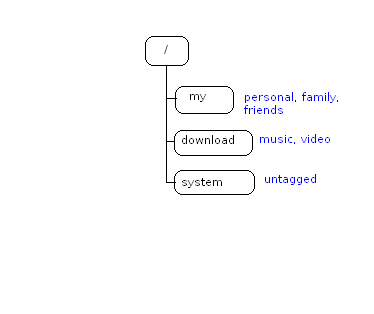
\includegraphics[scale=0.8]{art/schema.png}
\end{frame}

\section{Architecture}

\begin{frame}
  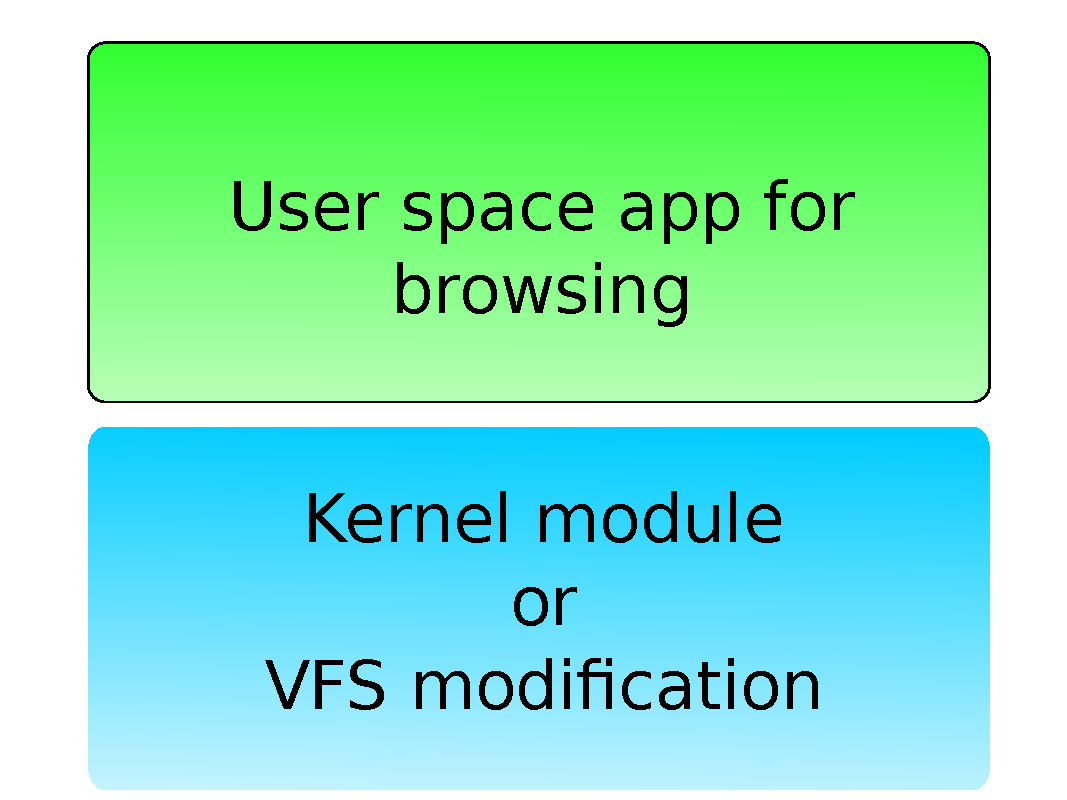
\includegraphics[scale=0.5]{art/archall.pdf}
\end{frame}

\begin{frame}
  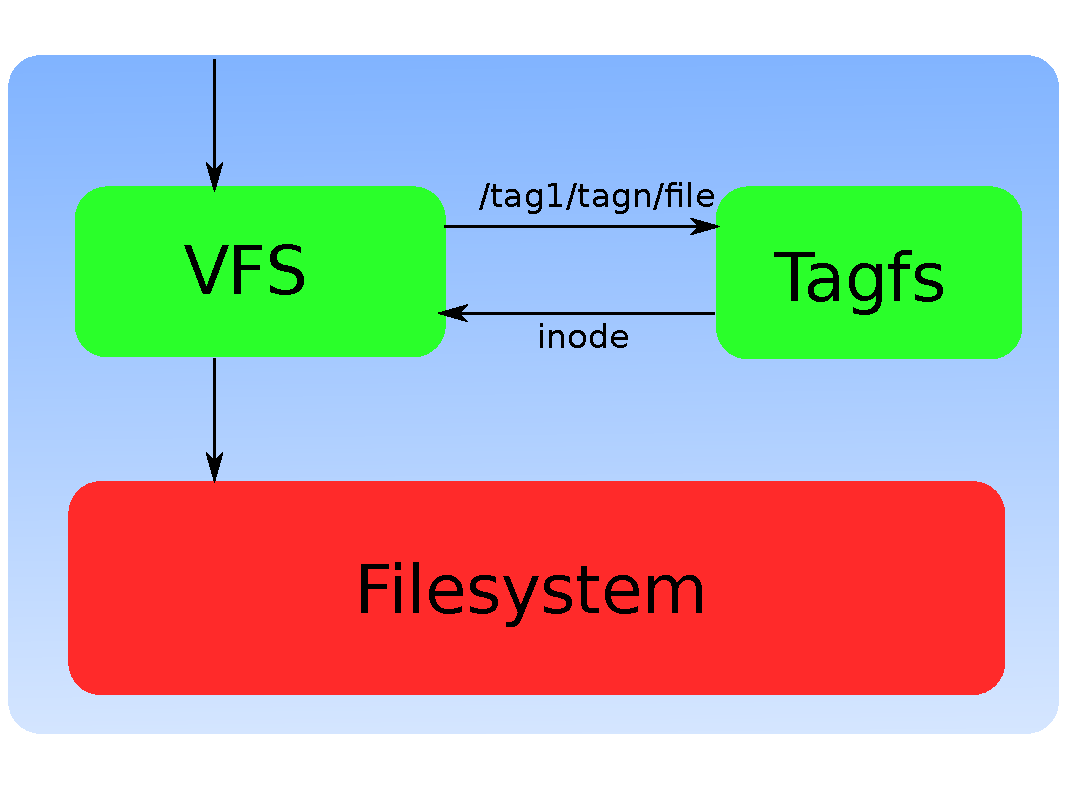
\includegraphics[scale=0.6]{art/archdetail.pdf}
\end{frame}

\section{Related work}

\begin{frame}
%\MyLogo  
  \begin{itemize}
  \item TagFS: Bringing Semantic Metadata to the Filesystem
    \begin{itemize}
    \item \url{http://www.eswc2006.org/poster-papers/FP31-Schenk.pdf}
    \end{itemize}
    
  \item Nepomuk
    \begin{itemize}
    \item \url{http://nepomuk.semanticdesktop.org/xwiki/bin/view/Main1/Deliverables}
    \end{itemize}
    
  \item Keywords: metadata, database
  \end{itemize}
  
\end{frame}

\section{Current status}

\begin{frame}
  \begin{itemize}
  \item Studied related work
  \item Stated expected behaviour
    \begin{itemize}
        \item Add, remove tags
        \item Find files based on tags
    \end{itemize}
  \item Identified pros and cons for the two possible solutions
    %\begin{itemize}
    %\item maybe listing a couple of + - for every solution,maybe we
    %  can make 2 slides out of this
    %\end{itemize}
  \end{itemize}
\end{frame}

\section{Employed Technologies}

\begin{frame}
  \begin{itemize}
  \item Linux 2.6.35
  \item GCC 4.4.5:
  \item FUSE  Filesystem in USErspace
	\begin{itemize}
	\item implement fully functional filesystem in a userspace program 
	\item piece of code that communicates with the kernel as a filesystem would
	\item runs on Linux kernels 2.4.X and 2.6.X
    \item libfuse - http://fuse.sourceforge.net/
    \end{itemize}
  \item C programming language
  \end{itemize}
\end{frame}

\section{Short term planning}

\begin{frame}
  \begin{itemize}
    \item Determine if VFS implementation is feasible
    \item Data organization
    \item Search methods
    \item Start coding
  \end{itemize}
\end{frame}

\section{Keywords}
\begin{frame}{Thank you!} 
\begin{columns}
	\begin{column}[l]{0.5\textwidth}
	  \begin{itemize}
        \item Filesystem
        \item Tags
        \item Inode
	  \end{itemize}
	\end{column}
	\begin{column}[c]{0.5\textwidth}
	  \begin{itemize}
        \item FUSE 
        \item VFS
	  \end{itemize}    
	\end{column}
      \end{columns}

\end{frame}
\end{document}
